\documentclass[10pt,a4paper]{article}

% ---------------------------------------------------------------- packages
\usepackage[T1]{fontenc}
\usepackage[utf8]{inputenc}
\usepackage{helvet}
\renewcommand{\familydefault}{\sfdefault}
\usepackage[a4paper,margin=1.8cm,top=1.5cm,bottom=1.8cm]{geometry}
\usepackage{graphicx}
\usepackage{booktabs}
\usepackage{tabularx}
\usepackage{array}
\usepackage{amsmath,amssymb}
\usepackage{caption}
\usepackage{float}
\usepackage{enumitem}
\usepackage{titlesec}
\usepackage[hidelinks,colorlinks=true,urlcolor=blue!70!black,linkcolor=black,citecolor=black]{hyperref}

\captionsetup{font=footnotesize,labelfont=bf,skip=3pt}
\titleformat{\section}{\large\bfseries}{\thesection.}{0.5em}{}
\titleformat{\subsection}{\normalsize\bfseries}{\thesubsection}{0.5em}{}
\titlespacing*{\section}{0pt}{8pt}{3pt}
\titlespacing*{\subsection}{0pt}{6pt}{2pt}
\setlength{\parindent}{0pt}
\setlength{\parskip}{4pt}
\setlength{\textfloatsep}{8pt}
\setlength{\floatsep}{8pt}
\newcolumntype{L}{>{\raggedright\arraybackslash}X}
\newcommand{\hyp}[2]{\par\hangindent=1em\hangafter=0\noindent\textbf{#1} #2\par}

% ----------------------------------------------------- EDIT TEAM / REPO
\newcommand{\repo}{https://github.com/hariharateja/ET610_ASSIGNMENT2}

\begin{document}

% =================================================================== title
\begin{center}
{\LARGE\bfseries Modelling Learner Behaviour Over Time:\\[2pt]
Engagement, Self-Regulation and At-Risk Prediction\\[2pt] in OULAD and Moodle\par}
\vspace{8pt}
\begin{tabular}{ll}
\toprule
\textbf{Team member} & \textbf{Roll number} \\
\midrule
Hari Hara Teja & 24b0977 \\
T Ganesh & 24b2250 \\
\bottomrule
\end{tabular}

\vspace{4pt}
{\small Code \& notebooks: \url{\repo} \quad$\cdot$\quad Submitted 5 October 2026}
\end{center}

\noindent\textbf{Abstract.} We analyse two learning-analytics datasets. One is the Open University Learning
Analytics Dataset (OULAD; 29,496 enrolments, 10.6\,M daily click records). The other is a 146,048-event Moodle log
from a blended IT course (161 learners). For each dataset we test hypotheses about early engagement, regularity,
self-monitoring and procrastination. We build weekly behavioural trajectories and evaluate supervised and
unsupervised models. In OULAD, a Random Forest trained on 2013 cohorts flags at-risk learners in the 2014 cohorts
with ROC-AUC 0.76 at week 4, 0.81 at week 8 and 0.93 at week 26. Regularity features add up to +0.07 AUC over click
volume. Submission latency, however, has no effect once score and submission rate are controlled for. In Moodle,
behaviour from the first ten weeks predicts completion of the final project (AUC 0.94). The strongest signals are
early Synopsis submission and self-monitoring of grades and feedback, not raw activity. K-Means separates four
profiles whose completion rates range from 8\% to 86\%.

% ============================================================ 1. intro
\section{Introduction \& Hypotheses}
Learning-management-system logs record what learners do and when they do it. Self-regulated learning theory
\cite{zimmerman2002} holds that successful learners plan, monitor and adjust their study. Procrastination research
\cite{steel2007} links delay to worse outcomes. Both theories predict that \emph{how} and \emph{when} a learner
engages matters, not only \emph{how much}. We ask three questions.
\textbf{RQ1:} How early do the trajectories of successful and unsuccessful learners diverge?
\textbf{RQ2:} Do timing behaviours (submission latency, regularity, self-monitoring) carry information beyond
activity volume?
\textbf{RQ3:} Can learners be segmented into interpretable behavioural profiles that differ in outcome?

\textbf{OULAD hypotheses.}
\hyp{O-H1 (early at-risk divergence).}{Learners who later fail or withdraw already show lower and declining VLE
engagement in the first weeks. Early clickstream features alone reach AUC $\geq$ 0.75 by week 4.}
\hyp{O-H2 (submission latency).}{Later submission relative to the deadline is associated with failing or
withdrawing, even after controlling for assessment score and submission rate.}
\hyp{O-H3 (regularity over volume).}{Engagement regularity (active-day and active-week ratios, weekly burstiness,
recency, activity diversity) adds predictive value beyond total clicks and demographics.}

\textbf{Moodle hypotheses.}
\hyp{M-H1 (distributed, self-monitored engagement).}{In weeks 0--9, learners who go on to submit the Final project
log in on more distinct days and weeks, have more regular gaps between sessions, and check their own grades and
feedback more often.}
\hyp{M-H2 (procrastination \& self-testing).}{Learners who submit the first milestone (Synopsis) close to its
deadline, or not at all, are less likely to complete the Final project. Completers also use practice quizzes more.
(The deadline is inferred from the data, so we test how early learners submit, not whether they submit late.)}
\hyp{M-H3 (behavioural profiles).}{Unsupervised clustering yields distinct, interpretable profiles (e.g.\ steady
self-regulators vs.\ exam-window-only users) with different completion rates.}

% ============================================================= 2. data
\section{Datasets \& Preprocessing}
\subsection{OULAD}
OULAD \cite{kuzilek2017} covers 22 presentations of 7 modules (2013--2014). It contains demographics, registration
dates, assessment deadlines and submissions, and daily click counts per VLE resource. Cleaning steps:
(i) we de-duplicated enrolments on (module, presentation, student).
(ii) We removed 3,097 enrolments that unregistered on or before day 0, because they never had a chance to engage.
This leaves 29,496 enrolments (Pass 12,361; Fail 7,044; Withdrawn 7,067; Distinction 3,024).
(iii) We joined click records to activity types and aggregated them to one row per enrolment and day.
(iv) We excluded exam rows from the assessment features, since exam dates are often missing. Banked (carried-over)
results were also dropped.
(v) Missing IMD bands and registration dates were imputed with the median.
The binary target is \textbf{at-risk = Fail or Withdrawn}. To mimic a real early-warning system, every feature at
cut-off day $c$ uses only events dated before $c$. Learners who had already withdrawn by $c$ are not predicted at
that cut-off.

\subsection{Moodle interaction log}
The Moodle export has 146,048 events for course IT-2507 (23 Oct 2025 -- 29 Jul 2026). Each event records a user, a
timestamp, an event context, a component, a content code and a description.
\textbf{Clean-up:} (i) for 3,334 SCORM events the \emph{User ID} column was truncated (e.g.\ \texttt{e id '3}). We
recovered the true id from the description text with a regular expression. (ii) We parsed the dd/mm/yy timestamps
and checked for exact duplicates (none found). (iii) We dropped 11 accounts with fewer than 30 events, leaving 161
learners. (iv) We excluded \emph{Quiz attempt auto-saved} events (37k rows) from action counts, because they are
system-generated during quiz attempts. They are kept for session timing.
\textbf{Sessionisation:} events from the same user less than 30 minutes apart belong to one session
\cite{kovanovic2015}. This gives 6,348 sessions (median 4 events, 1.5\,min). A single-event session is credited with
1 minute of time on task.
\textbf{Outcome \& leakage control:} the log contains no grades. Our outcome is therefore \textbf{submission of the
Final course-project assignment} (58 of 161 learners, 36\%). Predictive features use only events before 29 Dec 2025,
the day of the first Final submission. That gives an early window of weeks 0--9, from which all Final-assignment
events are removed. The Synopsis deadline is inferred as end of day 30 Nov 2025, the date of the last Synopsis
submission. Because of this, no submission can be late by construction (the closest one came 0.2 days before the
proxy deadline).

% ========================================================= 3. features
\section{Feature Extraction \& Engineering}
\begin{table}[H]
\centering\footnotesize
\begin{tabularx}{\textwidth}{>{\raggedright\arraybackslash}p{2.6cm}LL}
\toprule
\textbf{Construct} & \textbf{OULAD features (computed before cut-off $c$)} & \textbf{Moodle features (weeks 0--9)} \\
\midrule
Volume & log total clicks; log pre-start clicks & log actions; log content views (book, page, SCORM, video, PPT\ldots) \\
Regularity / time management & active days; active-day ratio (= active days / $c$); active-week ratio; weekly
coefficient of variation (burstiness); days since last login; recent trend (log clicks of last 2 weeks vs.\ earlier)
& sessions; active days; active-week ratio; weekly CV; SD of inter-session gaps; night (00--06\,h) and weekend share \\
Time on task & --- & total sessionised hours; mean session length (min) \\
Breadth / strategy & Shannon entropy of clicks across 20 activity types & distinct items accessed; practice-quiz
attempts \& share of actions; forum/glossary views \\
Submission behaviour & assessments due; submission rate; mean latency (days submitted $-$ deadline); mean score &
Synopsis submitted (0/1); Synopsis lead time (days before deadline; $-5$ if not submitted) \\
Self-monitoring & --- & views of own grade report, assignment feedback and submission status \\
Performance / context & prior attempts, credits, IMD band, education, age, gender, disability, registration day &
mean SCORM self-check score \\
\bottomrule
\end{tabularx}
\caption{Engineered features, grouped by behavioural construct. Clustering also uses an \emph{exam-window share}
feature: the share of a learner's actions in weeks 14--15 (26 Jan -- 8 Feb 2026, when the continuous-evaluation
quizzes ran).}
\end{table}

% ========================================================= 4. temporal
\section{Temporal Behavioural Visualisations}
\subsection{OULAD}
\begin{figure}[H]
\centering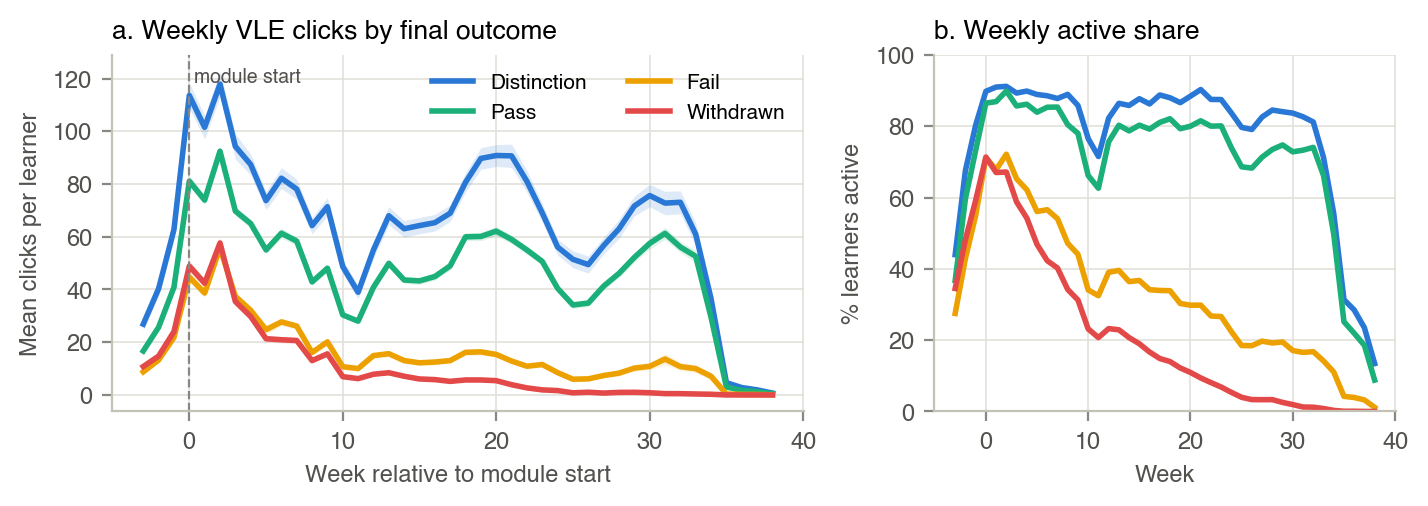
\includegraphics[width=\textwidth]{figures/oulad_weekly_clicks.png}
\caption{(a) Mean weekly VLE clicks per learner by final outcome (bands = 95\% CI). (b) Share of learners active in
each week. Week 0 is the module start.}
\end{figure}

All four groups engage strongly in the first fortnight, but the curves separate almost immediately (Fig.~1). In
week 0 the median at-risk learner logs 16 clicks, against 49 for successful learners (rank-biserial $r = 0.30$). By
week 4 the medians are 5 vs.\ 38 ($r = 0.40$). By week 6 the median at-risk learner is no longer active at all
($r = 0.47$). Two patterns stand out. Failing learners do not drop out: their activity stays low and gently
declining. Withdrawn learners decay steadily. Successful learners follow a periodic rhythm, with peaks around
weeks 2, 20 and 30 (assessment dates differ between modules, so these are pooled peaks). Both Distinction and Pass learners dip in week 11, which looks like a
scheduled break rather than disengagement.

\begin{figure}[H]
\centering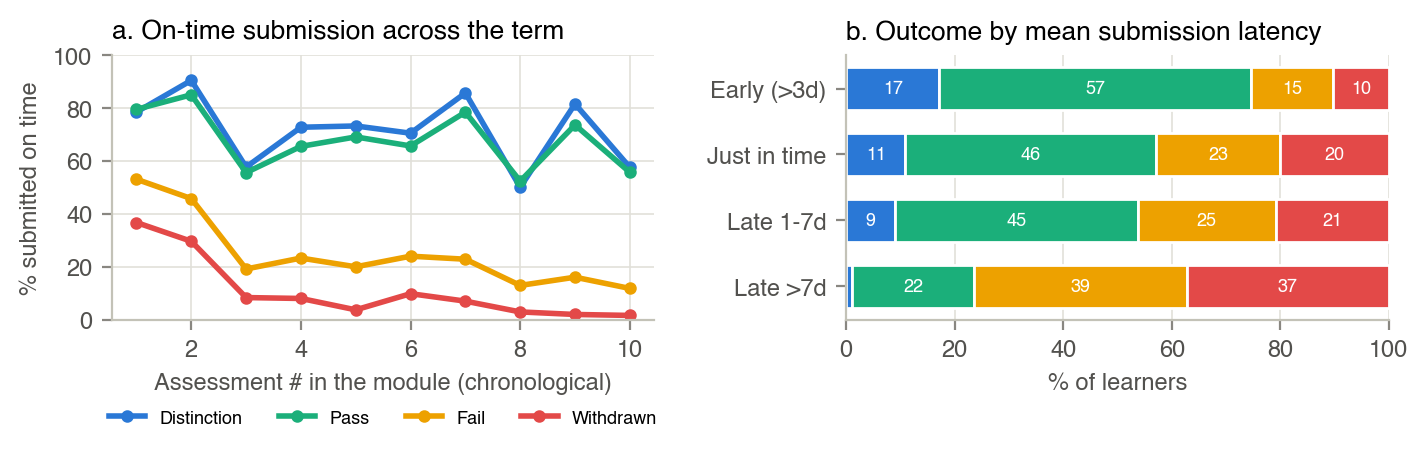
\includegraphics[width=\textwidth]{figures/oulad_latency.png}
\caption{(a) Share of each assessment submitted on or before its deadline, in chronological order within the
module. (b) Final-outcome mix by a learner's mean submission latency (submitted assessments only).}
\end{figure}

Submission punctuality (Fig.~2a) shows the same early separation. On the first assessment, at-risk groups are
already 26--42 points behind. By the third assessment fewer than 20\% of their assessments are submitted on time, partly
because many are never submitted. Mean latency is clearly graded with outcome (Fig.~2b): 25\% of learners who submit
more than 3 days early are at risk, against 76\% of those who are on average more than a week late (Spearman
$\rho = 0.24$).

\subsection{Moodle}
\begin{figure}[H]
\centering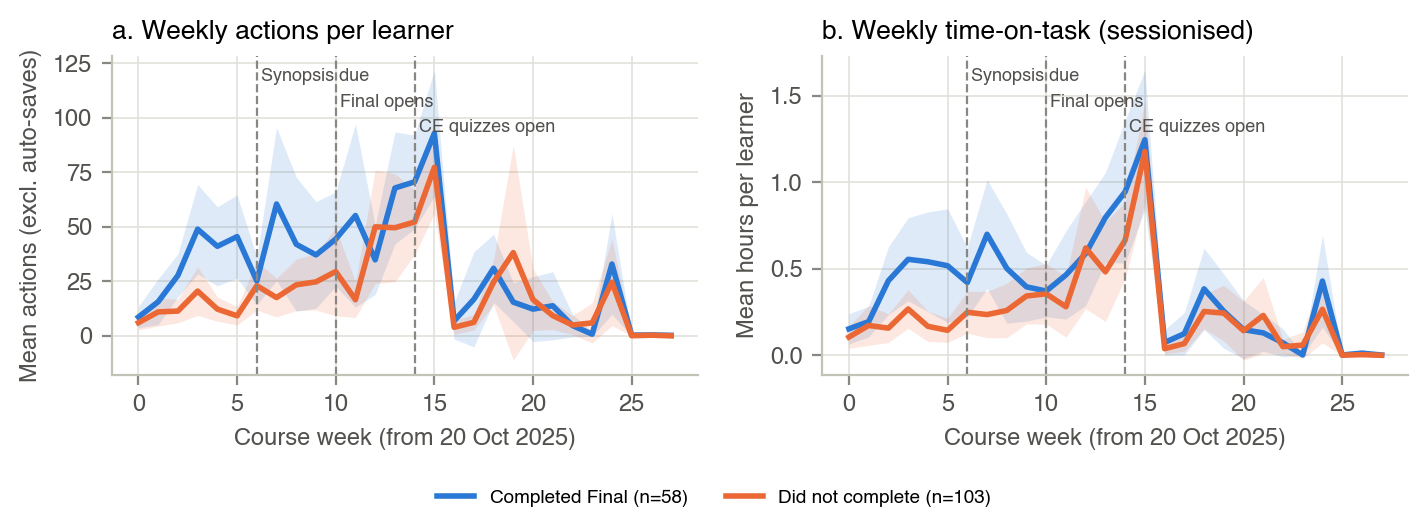
\includegraphics[width=\textwidth]{figures/moodle_weekly.png}
\caption{Weekly actions (a) and sessionised time-on-task (b) for learners who did and did not complete the Final
project (bands = 95\% CI). Dashed lines mark the Synopsis deadline, the opening of Final submissions and the
continuous-evaluation (CE) quiz window.}
\end{figure}

Completers are about twice as active as non-completers through the first ten weeks (Fig.~3). In weeks 2--5 they
spend roughly 0.5\,h per week on the platform, against about 0.2\,h. About a week after the Synopsis deadline
(week 7), completers produce a second burst of activity. The gap then closes. In the CE quiz window (weeks 14--15)
both groups converge on the same exam-driven peak, and after week 16 their trajectories are indistinguishable. In
short, the groups differ in when they engage, not in their exam-time effort: non-completers engage mainly when
assessment forces them to.

\begin{figure}[H]
\centering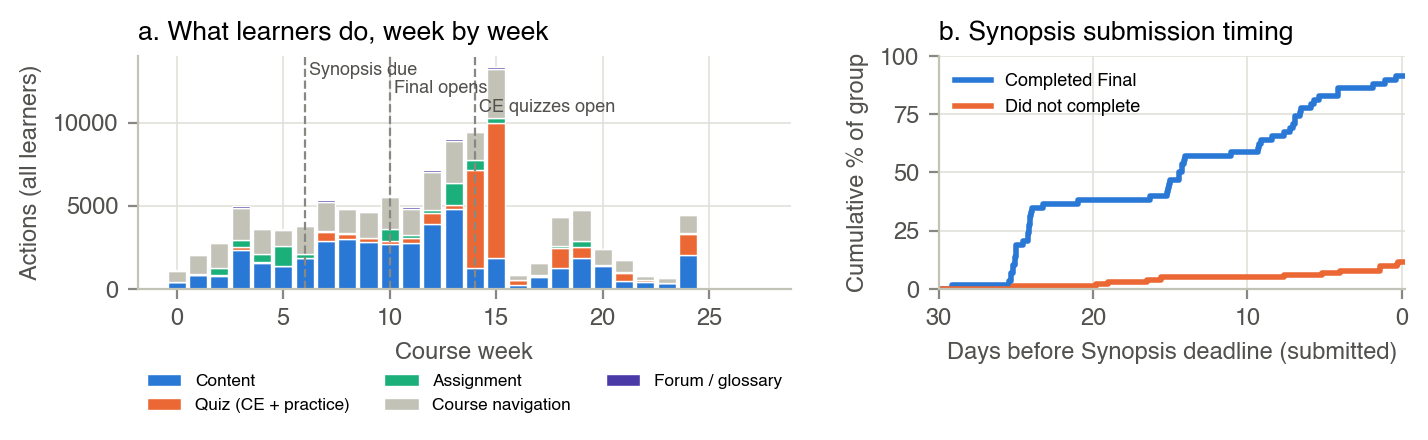
\includegraphics[width=\textwidth]{figures/moodle_mix_synopsis.png}
\caption{(a) Weekly composition of all learner actions by component (auto-saves excluded). (b) Cumulative share of
each group that had submitted the Synopsis, by days before its deadline (read left to right as time passes).}
\end{figure}

Figure~4a shows how activity moves through the course: content reading in weeks 3--13, assignment work around each
milestone, and a sharp switch to quizzes in weeks 14--15. Figure~4b shows the strongest temporal signal. About a
third (33\%) of eventual completers submitted the Synopsis more than 24 days early, and about 90\% submitted it before the
deadline. Only about 11\% of non-completers ever submitted it.

% ================================================================ 5. ML
\section{Machine Learning \& Results}
\subsection{OULAD --- early-warning classification (O-H1, O-H3) and trajectory clustering}
\textbf{Setup.} We compare L2 logistic regression (standardised, class-balanced) with a Random Forest (300 trees,
min leaf 10, balanced class weights; \cite{breiman2001}). Both use scikit-learn \cite{pedregosa2011}. Validation is
\textbf{temporal}: we train on all 2013 presentations and test on all 2014 presentations, so the model always
predicts a later cohort. We repeat this at nine cut-offs (weeks 1--26), each with three nested feature sets
(Table~1). We also ran 5-fold stratified cross-validation within the 2013 data at week 8 (RF AUC
0.827 $\pm$ 0.006). It is close to the temporal test score, so the model generalises across years.

\begin{figure}[H]
\centering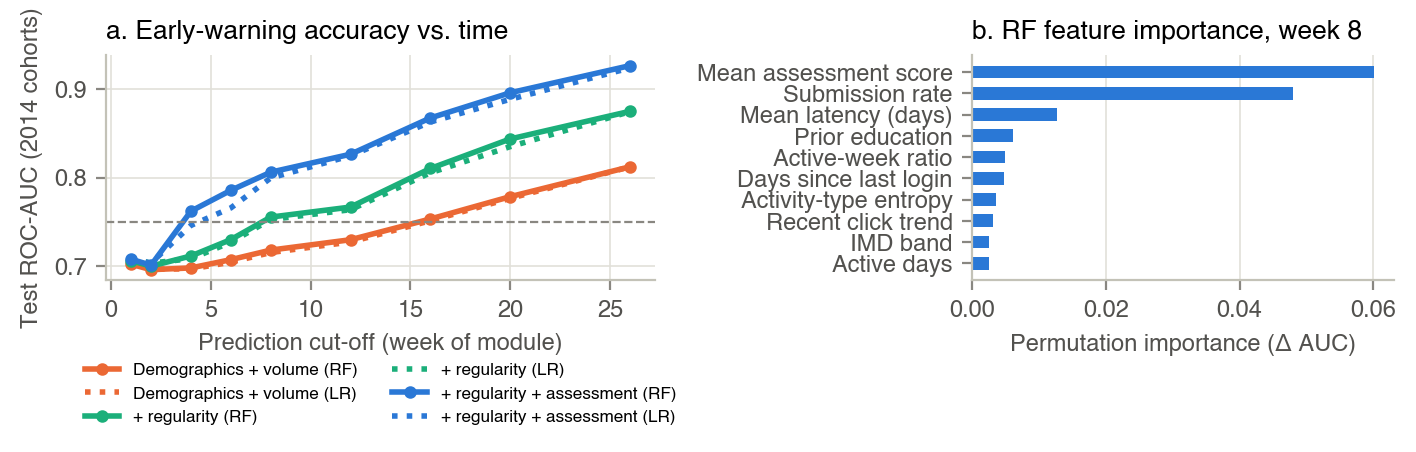
\includegraphics[width=\textwidth]{figures/oulad_ml.png}
\caption{(a) Test ROC-AUC on 2014 cohorts by prediction cut-off and feature set (solid = Random Forest, dotted =
logistic regression; dashed line = 0.75 target). (b) Permutation importance (drop in AUC) for the week-8 RF.}
\end{figure}

\begin{table}[H]
\centering\footnotesize
\begin{tabularx}{\textwidth}{Lccccc}
\toprule
\textbf{Model (week 8, 2014 test, $n$ = 15,098)} & \textbf{ROC-AUC} & \textbf{F1} & \textbf{Precision} & \textbf{Recall} & \textbf{Balanced acc.} \\
\midrule
Logistic regression (all features) & 0.800 & 0.670 & 0.685 & 0.656 & 0.720 \\
Random Forest (all features)       & 0.806 & 0.680 & 0.673 & 0.688 & 0.725 \\
RF, demographics + volume only     & 0.718 & & & & \\
RF, + regularity (no assessment)   & 0.755 & & & & \\
\bottomrule
\end{tabularx}
\caption{Week-8 early-warning performance (threshold 0.5; at-risk prevalence among learners still enrolled = 42\%).}
\end{table}

\textbf{Results.} Prediction accuracy rises steadily with time (Fig.~5a). With demographics and click volume only,
the RF reaches AUC 0.70 at week 4 and passes 0.75 only around week 16. Adding regularity features lifts AUC to 0.71
at week 4, 0.76 at week 8 and 0.88 at week 26. Adding assessment behaviour gives 0.76, 0.81 and 0.93. At week 8 the
RF identifies 69\% of at-risk learners at 67\% precision. Logistic regression is nearly as good, which suggests the
signal is largely monotonic. The most important week-8 features (Fig.~5b) are mean score, submission rate and
latency, followed by prior education, active-week ratio, recency and activity diversity. Total clicks matter much less once
regularity is known.

\textbf{O-H2 test.} We fitted a logistic regression of at-risk status on standardised mean latency, mean score and
submission rate ($n$ = 25,507 enrolments with $\geq$ 1 submission). Latency has \textbf{no independent effect} (OR per
SD = 1.00, 95\% CI 0.95--1.05, $p$ = 0.99). Score (OR 0.25) and submission rate (OR 0.06) are both highly
significant ($p < 0.001$).

\begin{figure}[H]
\centering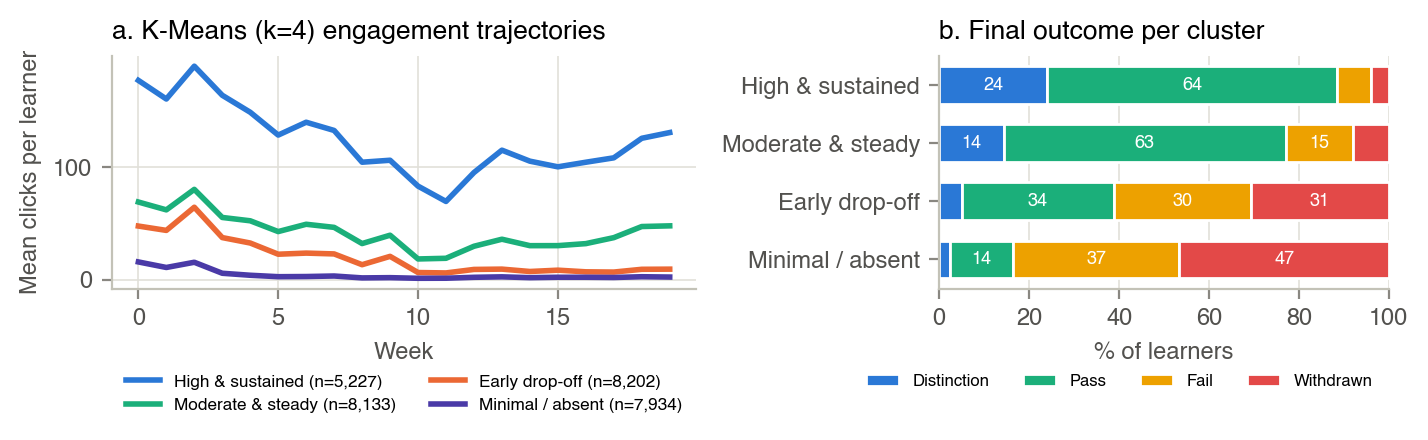
\includegraphics[width=\textwidth]{figures/oulad_clusters.png}
\caption{(a) Centroid trajectories from K-Means ($k = 4$) on log weekly clicks over weeks 0--19. (b) Final-outcome
mix within each cluster.}
\end{figure}

\textbf{Clustering.} We ran K-Means on log-transformed 20-week click trajectories. Silhouette favours $k = 2$
(0.33), a simple engaged/disengaged split. We report $k = 4$ (silhouette 0.18) because it separates the
\emph{timing} of disengagement. The four profiles are \emph{high \& sustained} (12\% at risk), \emph{moderate \&
steady} (23\%), \emph{early drop-off} (61\%) and \emph{minimal/absent} (84\%) (Fig.~6). The early drop-off cluster
starts at a similar level to the moderate cluster but falls away after week 3. These are the learners an
intervention could still reach.

\subsection{Moodle --- completion prediction (M-H1, M-H2) and profile discovery (M-H3)}
\textbf{Setup.} With $n = 161$, a single train/test split would be unstable. We therefore use \textbf{repeated
stratified 5-fold cross-validation (10 repeats, 50 folds)} and report mean $\pm$ SD. The models are an L2 logistic
regression ($C = 0.3$) and a Random Forest (400 trees, min leaf 3), both class-balanced. Two baselines put the
results in context: logistic regression on action count alone, and an RF without any submission-related or
self-monitoring features. Univariate group differences use Mann--Whitney $U$ tests with Holm correction across 19
features.

\begin{table}[H]
\centering\footnotesize
\begin{tabularx}{\textwidth}{Lccccc}
\toprule
\textbf{Model (weeks 0--9 features $\rightarrow$ Final submitted)} & \textbf{ROC-AUC} & \textbf{F1} & \textbf{Precision} & \textbf{Recall} & \textbf{Balanced acc.} \\
\midrule
Logistic regression (all 19 features) & 0.939 $\pm$ 0.045 & 0.849 $\pm$ 0.062 & 0.814 $\pm$ 0.079 & 0.895 $\pm$ 0.084 & 0.887 $\pm$ 0.050 \\
Random Forest (all 19 features)       & 0.943 $\pm$ 0.037 & 0.857 $\pm$ 0.063 & 0.832 $\pm$ 0.080 & 0.890 $\pm$ 0.081 & 0.892 $\pm$ 0.051 \\
RF, behaviour only (no Synopsis / self-monitoring) & 0.739 $\pm$ 0.078 & & & & \\
Baseline LR, action count only        & 0.725 $\pm$ 0.091 & & & & \\
\bottomrule
\end{tabularx}
\caption{Moodle cross-validated performance (mean $\pm$ SD over 50 folds).}
\end{table}

\begin{figure}[H]
\centering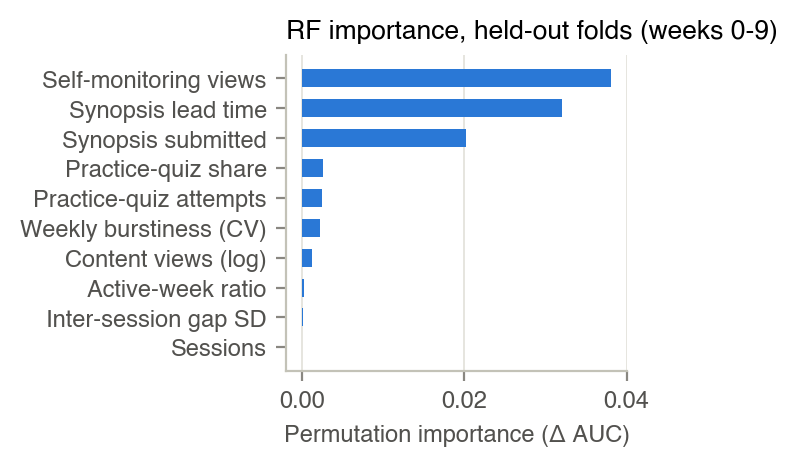
\includegraphics[width=0.5\textwidth]{figures/moodle_importance.png}
\caption{Random-Forest permutation importance, measured on held-out folds. Importance is costly to compute, so it
uses 20 folds (5-fold $\times$ 4 repeats) rather than the 50 folds (5-fold $\times$ 10 repeats) behind Table~3.}
\end{figure}

\begin{table}[H]
\centering\footnotesize
\begin{tabularx}{\textwidth}{Lcccc}
\toprule
\textbf{Feature (weeks 0--9)} & \textbf{Median: completed} & \textbf{Median: not} & \textbf{Rank-biserial $r$} & \textbf{Holm $p$} \\
\midrule
Synopsis lead time (days)   & 14.34 & $-5.00$ & $+0.84$ & $< 0.001$ \\
Self-monitoring views       & 16.00 & 0.00    & $+0.90$ & $< 0.001$ \\
Active days                 & 14.00 & 7.00    & $+0.53$ & $< 0.001$ \\
Inter-session gap SD (days) & 3.24  & 6.31    & $-0.51$ & $< 0.001$ \\
Active-week ratio           & 0.70  & 0.50    & $+0.50$ & $< 0.001$ \\
Sessions                    & 17.00 & 8.00    & $+0.49$ & $< 0.001$ \\
Time on task (h)            & 3.10  & 1.08    & $+0.43$ & $< 0.001$ \\
Practice-quiz share         & 0.00  & 0.00    & $+0.05$ & 1.00 \\
SCORM self-check score      & 40.58 & 40.58   & $-0.00$ & 1.00 \\
\bottomrule
\end{tabularx}
\caption{Selected univariate comparisons between completers ($n$ = 58) and non-completers ($n$ = 103). Note:
learners who never submitted the Synopsis are assigned a lead time of $-5$ days. The non-completer median of
$-5.00$ is therefore this imputed value (most non-completers never submitted), not an observed lead time.}
\end{table}

\textbf{Results.} Both models predict Final completion from week-0--9 behaviour with AUC $\approx$ 0.94 (Table~3).
However, Fig.~7 and the behaviour-only ablation show that the signal is concentrated in the Synopsis features
(whether and how early it was submitted) and in self-monitoring. Removing them drops AUC to 0.74, barely above the action-count baseline (0.73). The
univariate tests (Table~4) still support M-H1. Completers were active on twice as many days, had more regular gaps
between sessions ($r = -0.51$) and checked their grades and feedback far more often ($r = +0.90$). M-H2 is split. We
grouped Synopsis timing into four categories and counted Final completers in each: not submitted, 5 of 96; less
than 1 day before the deadline, 1 of 3; 1--7 days before, 11 of 15; more than 7 days before, 41 of 47. The
$4 \times 2$ table gives $\chi^2(3) = 102$, $p < 0.001$. Practice-quiz use, by contrast, did not differ between groups
(Holm $p$ = 1.00).

\begin{figure}[H]
\centering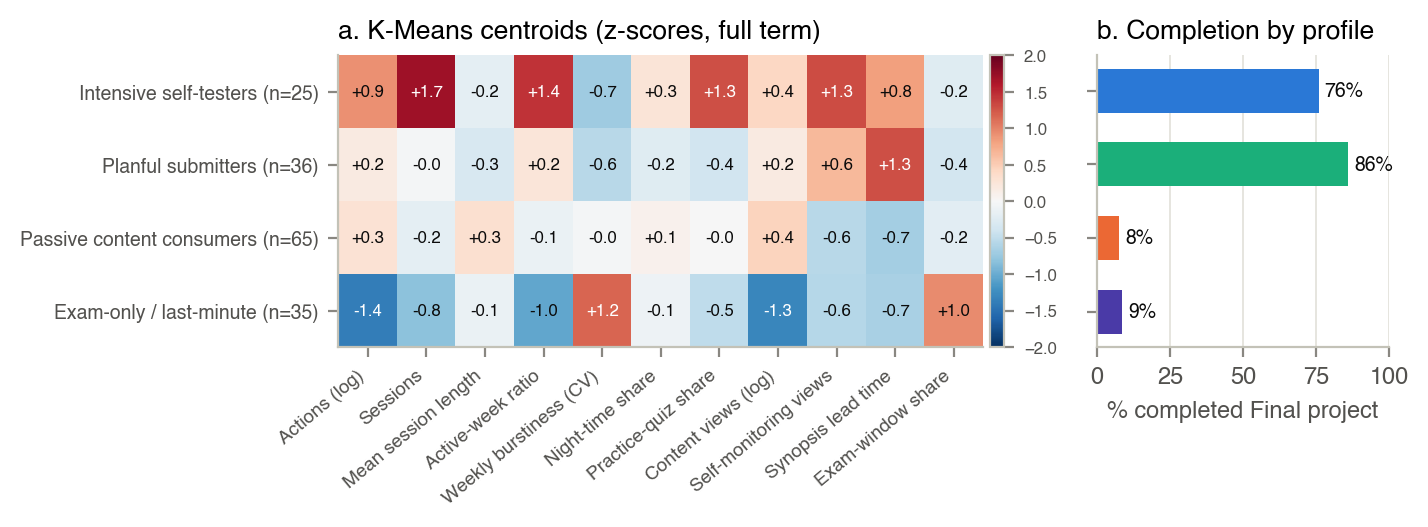
\includegraphics[width=\textwidth]{figures/moodle_clusters.png}
\caption{(a) K-Means ($k = 4$) centroids on 11 standardised whole-term features (red = above cohort mean).
(b) Share of each profile that completed the Final project. The Synopsis lead-time column includes the $-5$-day value assigned to non-submitters. Features cover the whole term, including the period after the outcome, so the profiles describe behaviour and do not predict it.}
\end{figure}

\textbf{Profiles (M-H3).} K-Means on 11 standardised whole-term features (Fig.~8) produced four interpretable
groups. \emph{Intensive self-testers} ($n$ = 25) have the most sessions, the most active weeks and the heaviest
practice-quiz use (76\% completed). \emph{Planful submitters} ($n$ = 36) are only moderately active but submit very
early (17 days ahead) and check feedback (86\% completed). \emph{Passive content consumers} ($n$ = 65) read as much
material as anyone, in longer sessions, but rarely submit or self-monitor; only 8\% completed. \emph{Exam-only / last-minute}
learners ($n$ = 35) put 46\% of all their activity into the two CE weeks; only 9\% completed the Final. Completion differs strongly across
clusters ($\chi^2$ $p < 0.001$). Silhouette values are low, however (between 0.18 and 0.21 for every $k$ from 2 to 7). The
profiles are best read as regions of a continuum rather than sharply separated types.

% ======================================================= 6. discussion
\section{Discussion \& Conclusion}
\begin{table}[H]
\centering\footnotesize
\begin{tabularx}{\textwidth}{>{\raggedright\arraybackslash}p{3.3cm}>{\raggedright\arraybackslash}p{2.6cm}L}
\toprule
\textbf{Hypothesis} & \textbf{Verdict} & \textbf{Key evidence} \\
\midrule
O-H1 early divergence & Supported (partly) & Trajectories separate from week 0 ($r$ = 0.30, rising to 0.47 by week 6).
Without assessment data (demographics + clickstream), AUC at week 4 = 0.71 ($<$ 0.75); 0.75 is reached by week 8 (0.76), or by week 4 once assessment
data are added (0.76). \\
O-H2 latency & Not supported (independently) & Strong bivariate gradient (25\% $\rightarrow$ 76\% at risk), but
OR = 1.00 after controlling for score and submission rate. \\
O-H3 regularity & Supported & +0.04 AUC at week 8 and +0.06 at week 16 over volume. Active-week ratio and recency
outrank total clicks. \\
M-H1 distributed / self-monitoring & Supported & Active days, session regularity and self-monitoring all differ
(Holm $p < 0.001$). Self-monitoring is the top predictor. \\
M-H2 procrastination / self-testing & Partly supported & Early Synopsis submission strongly predicts completion and non-submission
predicts failure to complete ($\chi^2(3)$ $p < 0.001$). Lateness cannot be tested (inferred deadline).
Practice-quiz use does not differ ($p$ = 1.00). \\
M-H3 profiles & Supported (weak structure) & Four interpretable profiles; completion ranges from 8\% to 86\%.
Silhouette $\approx$ 0.18. \\
\bottomrule
\end{tabularx}
\caption{Summary of hypothesis tests.}
\end{table}

\textbf{Interpretation.} The two datasets tell the same story. \emph{When} and \emph{how regularly} learners engage
reveals more than how much they click, and the most informative behaviours involve meeting early milestones and
monitoring one's own progress. These are the behaviours that self-regulated learning theory points to. The OULAD
latency result is a useful caution. Late submission looks like a risk factor, but it adds nothing once the model
knows whether the learner submits at all and how well they score. Lateness appears to be a symptom of the same
underlying disengagement, not a separate cause.

\textbf{Implications for course design and automated intervention.}
(1) \emph{Intervene early, and use assessment data.} An OULAD-style alert at week 4 that combines regularity with
the first assessment already reaches AUC $\approx$ 0.76. Making the first assessment small and early therefore gives
the alert system data as well as giving learners practice.
(2) \emph{Monitor regularity, not volume.} Dashboards should show active weeks and days since the last login. A
learner with many clicks crammed into one week is not on track.
(3) \emph{Treat the first milestone as a sensor.} In Moodle, not submitting the Synopsis identified 91 of 103
eventual non-completers by 30 Nov, while flagging only 5 completers, four weeks before the Final opened. A
deadline-plus-48-hours nudge is a cheap, explainable trigger.
(4) \emph{Prompt self-monitoring.} Completers checked feedback and grade reports far more often. Pushing feedback to
learners and adding progress widgets may help the passive and exam-only groups adopt the habit. Whether this would
change outcomes is causal and should be tested with an A/B design.

\textbf{Limitations.} Our analyses are correlational. The Moodle outcome is project completion, not a grade, and the
cohort is a single course of 161 learners. Synopsis and self-monitoring features are close in kind to the outcome
itself, and the Synopsis deadline is inferred rather than taken from the course calendar. Time-on-task depends on the 30-minute session threshold. OULAD click counts do not record dwell time. Future
work could add sequence models (e.g.\ HMMs over weekly states), calibrate the alert thresholds to intervention
capacity, and audit fairness across IMD and disability groups before deployment.

% ======================================================== references
\begingroup
\footnotesize
\begin{thebibliography}{9}\setlength{\itemsep}{0pt}
\bibitem{breiman2001} Breiman, L. (2001). Random forests. \emph{Machine Learning}, 45(1), 5--32.
\bibitem{kovanovic2015} Kovanovi\'c, V., Ga\v{s}evi\'c, D., Dawson, S., Joksimovi\'c, S., Baker, R.\,S., \&
Hatala, M. (2015). Penetrating the black box of time-on-task estimation. \emph{Proc.\ LAK '15}, 184--193.
\bibitem{kuzilek2017} Kuzilek, J., Hlosta, M., \& Zdrahal, Z. (2017). Open University Learning Analytics dataset.
\emph{Scientific Data}, 4, 170171.
\bibitem{pedregosa2011} Pedregosa, F.\ et al.\ (2011). Scikit-learn: Machine learning in Python. \emph{JMLR}, 12,
2825--2830.
\bibitem{steel2007} Steel, P. (2007). The nature of procrastination. \emph{Psychological Bulletin}, 133(1), 65--94.
\bibitem{zimmerman2002} Zimmerman, B.\,J. (2002). Becoming a self-regulated learner: An overview. \emph{Theory Into
Practice}, 41(2), 64--70.
\end{thebibliography}
\endgroup

{\footnotesize\textbf{Appendix --- code.} All analysis is reproducible from \url{\repo}:
\texttt{code/oulad\_analysis.py} (OULAD pipeline, $\approx$ 1 min), \texttt{code/moodle\_analysis.py} (Moodle
pipeline), \texttt{code/build\_report.py} (PDF build); intermediate results are in \texttt{outputs/}.\par}

\end{document}
